\documentclass[aspectratio=169,11pt]{beamer}
\usepackage[T1]{fontenc}
\usepackage{lmodern}
\usepackage{amsmath,amssymb,booktabs,array,tikz}
\usetikzlibrary{arrows.meta,positioning,calc,fit,backgrounds}
\usefonttheme{professionalfonts}
\definecolor{ink}{HTML}{14263D}
\definecolor{blue}{HTML}{2463B4}
\definecolor{teal}{HTML}{167D8D}
\definecolor{coral}{HTML}{C6513E}
\definecolor{slate}{HTML}{687D94}
\definecolor{muted}{HTML}{52657A}
\definecolor{pale}{HTML}{F3F6FA}
\definecolor{edge}{HTML}{DCE4EE}
\colorlet{underfit}{slate}
\colorlet{wellfit}{blue}
\colorlet{overfit}{coral}
\setbeamercolor{normal text}{fg=ink,bg=pale}
\setbeamercolor{structure}{fg=blue}
\setbeamercolor{frametitle}{fg=ink}
\setbeamercolor{block title}{fg=blue,bg=blue!9}
\setbeamercolor{block body}{fg=ink,bg=white}
\setbeamerfont{frametitle}{size=\Large,series=\bfseries}
\setbeamerfont{block title}{size=\normalsize,series=\bfseries}
\setbeamertemplate{navigation symbols}{}
\setbeamertemplate{headline}{\textcolor{blue}{\rule{\paperwidth}{1.7mm}}}
\setbeamertemplate{footline}{\hspace{5mm}\scriptsize\color{muted}GUnit\quad iML 26/27\quad Feature effects in neural operators\hfill\insertframenumber\hspace{5mm}\vspace{3mm}}
\setbeamersize{text margin left=6mm,text margin right=6mm}
\setlength{\abovedisplayskip}{4pt}
\setlength{\belowdisplayskip}{4pt}
\newcommand{\key}[1]{\par\vspace{1mm}\begin{beamercolorbox}[sep=1.7mm,wd=\textwidth]{block title}\small\bfseries #1\end{beamercolorbox}}
\newcommand{\smallnote}[1]{\par\vspace{0.5mm}{\scriptsize\color{muted}#1}}
\newcommand{\goal}[1]{{\small\color{blue}\textbf{Goal:} #1}\par\vspace{1mm}}
\newcommand{\asset}[2]{\includegraphics[width=#2\textwidth]{generated/#1.pdf}}
\tikzset{box/.style={draw=edge,fill=white,rounded corners=2mm,align=center,inner sep=2mm},
 flow/.style={-{Stealth[length=2mm]},draw=muted,thick},
 learn/.style={box,draw=blue,fill=blue!6},
 temporal/.style={box,draw=teal,fill=teal!6}}
\newcommand{\ScoreRows}{\textcolor{underfit}{Underfit} & 37.62\% & 37.20\% & 45.11\% & 46.90\% \\
\textcolor{wellfit}{Well-fit} & 0.69\% & 3.08\% & 0.40\% & 0.45\% \\
\textcolor{overfit}{Overfit} & 0.08\% & 3.87\% & 0.36\% & 1.44\% \\}
\newcommand{\ConfigRows}{FNO & \textcolor{underfit}{Underfit} & 2 & 1 & 1 & 0.1 & 650 \\
FNO & \textcolor{wellfit}{Well-fit} & 16 & 8 & 2 & 0.002 & 1,400 \\
FNO & \textcolor{overfit}{Overfit} & 48 & 16 & 3 & 0 & 2,200 \\
LNO & \textcolor{underfit}{Underfit} & 2 & 1 & 1 & 0.1 & 650 \\
LNO & \textcolor{wellfit}{Well-fit} & 8 & 8 & 1 & 0 & 3,500 \\
LNO & \textcolor{overfit}{Overfit} & 48 & 16 & 3 & 0 & 3,500 \\}
\newcommand{\CountRows}{FNO & \textcolor{underfit}{Underfit} & nonlinear & 37 \\
FNO & \textcolor{wellfit}{Well-fit} & nonlinear & 9,137 \\
FNO & \textcolor{overfit}{Overfit} & nonlinear & 230,977 \\
LNO & \textcolor{underfit}{Underfit} & nonlinear & 43 \\
LNO & \textcolor{wellfit}{Well-fit} & linear & 537 \\
LNO & \textcolor{overfit}{Overfit} & nonlinear & 26,065 \\}

\title{Can we trust a model's explanations?}
\author{GUnit}
\begin{document}

% MAIN 1 -- 15 seconds
\begin{frame}{Learn a solution operator, then explain it}
{\small\textbf{Presented by GUnit}}\par\vspace{1mm}
\goal{Predict a complete physical solution from an input function and its parameters.}
\begin{center}
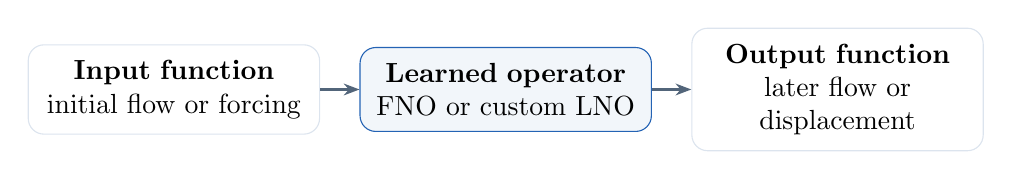
\begin{tikzpicture}[node distance=5mm]
\node[box,text width=33mm] (in) {\textbf{Input function}\\initial flow or forcing};
\node[learn,text width=33mm,right=of in] (model) {\textbf{Learned operator}\\FNO or custom LNO};
\node[box,text width=33mm,right=of model] (out) {\textbf{Output function}\\later flow or displacement};
\draw[flow] (in)--(model);\draw[flow] (model)--(out);
\end{tikzpicture}
\end{center}
\begin{columns}[T,onlytextwidth]
\column{.48\textwidth}\begin{block}{Prediction question}\small How accurately does the model reproduce the simulator's solution?\end{block}
\column{.48\textwidth}\begin{block}{Explanation question}\small How does changing viscosity or forcing frequency change predicted solution strength?\end{block}
\end{columns}
\key{We compare underfit, well-fit and overfit configurations on the same physical task.}
\end{frame}

% MAIN 2 -- 20 seconds
\begin{frame}{FNO task: initial flow $\longrightarrow$ later flow}
\goal{Learn the periodic Burgers solution map at final time $T=1$.}
\begin{columns}[T,onlytextwidth]
\column{.53\textwidth}
\begin{block}{Physical problem}
\[\frac{\partial u}{\partial t}+u\frac{\partial u}{\partial s}
 =\nu\frac{\partial^2u}{\partial s^2}\]
\small Periodic space $s\in[0,2\pi)$; viscosity $\nu$ controls diffusion.
\end{block}
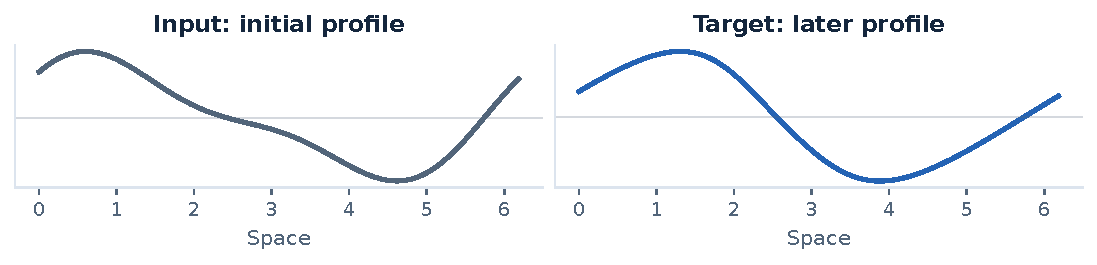
\includegraphics[width=\textwidth]{generated/burgers_io.pdf}
\column{.44\textwidth}
\begin{block}{Input: six channels on 64 spatial points}
\small Initial function $u_0(s)$; physical inputs $\nu,a,b,\phi$; spatial coordinate $s$.
\end{block}
\begin{block}{Output: 64 values of the later profile}
\[\widehat u(s,1)=G_\theta(u_0,\nu,a,b,\phi)(s)\]
\small Training target: simulator solution $u(s,1)$.
\end{block}
\end{columns}
\smallnote{Initial family: $u_0(s)=a\sin(s+\phi)+b\cos(2s-\phi)$. Plotted curves are simulator input and target.}
\key{The FNO predicts the whole spatial profile. We later explain the effect of viscosity.}
\end{frame}

% MAIN 3 -- 20 seconds
\begin{frame}{FNO: Fourier neural operator}
\goal{Learn how spatial Fourier modes interact to predict the later solution.}
\begin{center}
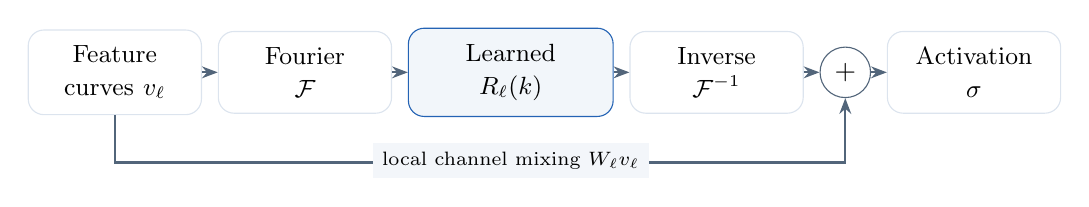
\begin{tikzpicture}[node distance=2mm]
\node[box,text width=18mm] (a) {\small Feature\\curves $v_\ell$};
\node[box,text width=18mm,right=of a] (b) {\small Fourier\\$\mathcal F$};
\node[learn,text width=22mm,right=of b] (c) {\small Learned\\$R_\ell(k)$};
\node[box,text width=18mm,right=of c] (d) {\small Inverse\\$\mathcal F^{-1}$};
\node[circle,draw=muted,fill=white,inner sep=1mm,right=of d] (sum) {$+$};
\node[box,text width=18mm,right=of sum] (e) {\small Activation\\$\sigma$};
\draw[flow](a)--(b);\draw[flow](b)--(c);\draw[flow](c)--(d);
\draw[flow](d)--(sum);\draw[flow](sum)--(e);
\draw[flow](a.south)--++(0,-6mm) -| (sum.south);
\node[fill=pale,font=\scriptsize,below=3.2mm of c] {local channel mixing $W_\ell v_\ell$};
\end{tikzpicture}
\end{center}
\vspace{1mm}
{\large\begin{equation*}
v_{\ell+1}=\sigma\!\left(W_\ell v_\ell+
\mathcal F^{-1}\!\left[R_\ell(k)\,\mathcal F(v_\ell)\right]\right)
\end{equation*}}
\begin{columns}[T,onlytextwidth]
\column{.49\textwidth}\begin{block}{Learned by optimization}\small Complex Fourier weights $R_\ell(k)$, local weights $W_\ell$, and input/output projections.\end{block}
\column{.48\textwidth}\begin{block}{Chosen before training}\small \textbf{Modes}: retained spatial frequencies.\\\textbf{Width}: hidden channels.\quad\textbf{Depth}: layers.\end{block}
\end{columns}
\smallnote{$v_\ell$ denotes hidden feature curves; $\sigma$ is GELU. Several layers sit between input lifting and output projection.}
\end{frame}

% MAIN 4 -- 20 seconds
\begin{frame}{LNO task: forcing history $\longrightarrow$ displacement}
\goal{Learn the forced, damped oscillator response over $0\leq t\leq12$.}
\begin{columns}[T,onlytextwidth]
\column{.53\textwidth}
\begin{block}{Physical problem}
\[\ddot x(t)+0.4\dot x(t)+4x(t)=f(t)\]
\[f(t)=A\cos(\omega t+\phi)\]
\small Initial conditions: $x(0)=x_0$, $\dot x(0)=0$.
\end{block}
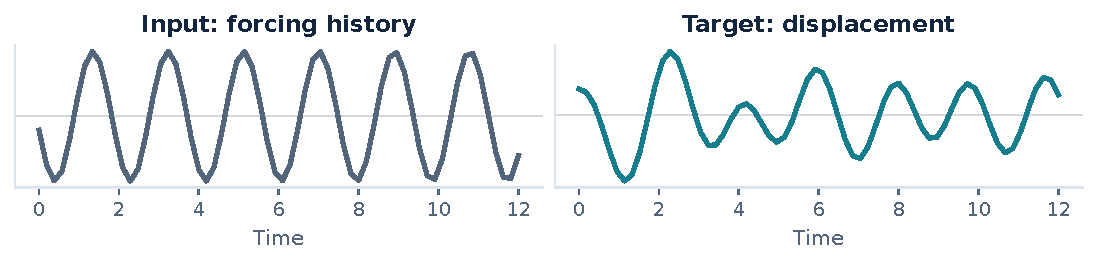
\includegraphics[width=.96\textwidth]{generated/oscillator_io.pdf}
\column{.44\textwidth}
\begin{block}{Input: six channels on 64 time points}
\small Forcing history $f(t)$; physical inputs $\omega,A,\phi,x_0$; time coordinate $t$.
\end{block}
\begin{block}{Output: 64 displacement values}
\[\widehat x(t)=G_\theta(f,\omega,A,\phi,x_0)(t)\]
\small Training target: simulator trajectory $x(t)$.
\end{block}
\end{columns}
\smallnote{Mass, damping and stiffness stay fixed: $m=1$, $c=0.4$, $k=4$. Plotted curves are simulator examples.}
\key{The LNO predicts the whole response history. We later explain forcing frequency.}
\end{frame}

% MAIN 5 -- 20 seconds
\begin{frame}{LNO: Laplace neural operator (custom)}
\goal{Learn decaying oscillatory memory: how past forcing affects the current response.}
\begin{center}
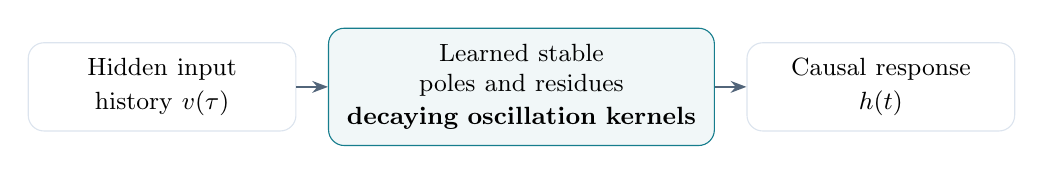
\begin{tikzpicture}[node distance=4mm]
\node[box,text width=30mm] (v) {\small Hidden input\\history $v(\tau)$};
\node[temporal,text width=45mm,right=of v] (k) {\small Learned stable poles and residues\\\textbf{decaying oscillation kernels}};
\node[box,text width=30mm,right=of k] (h) {\small Causal response\\$h(t)$};
\draw[flow](v)--(k);\draw[flow](k)--(h);
\end{tikzpicture}
\end{center}\vspace{-1.5mm}
{\large\begin{equation*}
K(t)=\sum_{j=1}^{P}e^{-\alpha_jt}
 \bigl[c_j\cos(\beta_jt)+d_j\sin(\beta_jt)\bigr],\qquad\alpha_j>0
\end{equation*}}
{\large\begin{equation*}
h(t)=\int_0^t K(t-\tau)\,v(\tau)\,\mathrm d\tau
\end{equation*}}
\begin{columns}[T,onlytextwidth]
\column{.49\textwidth}\small\textbf{Learned:} decay $\alpha_j$, frequency $\beta_j$, mixture coefficients $c_j,d_j$, and channel weights.
\column{.48\textwidth}\small\textbf{Chosen:} $P$ pole pairs per channel, hidden width and layer count.
\end{columns}
\smallnote{Laplace poles: $-\alpha_j\pm i\beta_j$. Local/channel mixing is also present.}
\key{Pole frequencies $\beta_j$ are learned; forcing frequency $\omega$ is a physical input.}
\end{frame}

% MAIN 6 -- 35 seconds
\begin{frame}{These settings create the three fit regimes}
\small\textbf{Model hyperparameters change; training data are matched within each refit.}
\vspace{1mm}
\begin{center}\small\renewcommand{\arraystretch}{1.18}
\begin{tabular}{llrrrrr}\toprule
Model & Regime & Width & Modes / pairs & Layers & Weight decay & Steps\\\midrule
\ConfigRows
\bottomrule\end{tabular}\end{center}
\begin{columns}[T,onlytextwidth]
\column{.49\textwidth}\begin{block}{Model settings control fit}\small Small width/mode count + stronger regularization restrict flexibility. Larger unregularized models can fit training details.\end{block}
\column{.48\textwidth}\begin{block}{Physical features define the task}\small Burgers: viscosity $\nu\in[0.06,0.25]$.\\Oscillator: forcing $\omega\in[0.5,3.5]$.\\These are \textbf{inputs}, not capacity settings.\end{block}
\end{columns}
\smallnote{Well-fit LNO uses a linear stack; other LNOs are nonlinear. Nonlinear overfit LNO uses cosine learning-rate decay.}
\end{frame}

% MAIN 7 -- 30 seconds
\begin{frame}{Controlled protocol: train, explain and verify}
\begin{center}
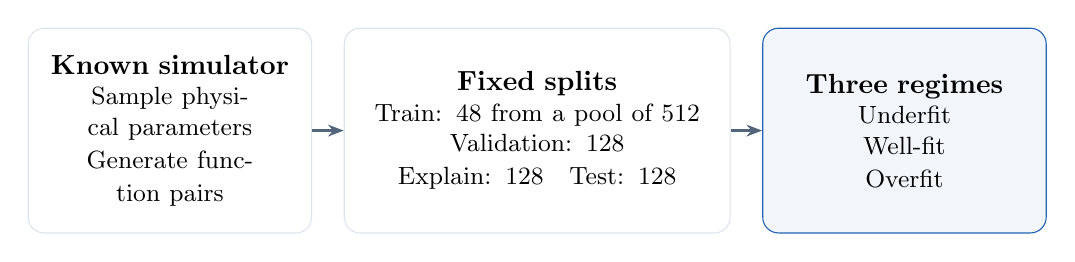
\begin{tikzpicture}[node distance=4mm]
\node[box,text width=32mm,minimum height=26mm] (sim) {\textbf{Known simulator}\\\small Sample physical parameters\\Generate function pairs};
\node[box,text width=45mm,minimum height=26mm,right=of sim] (split) {\textbf{Fixed splits}\\\small Train: 48 from a pool of 512\\Validation: 128\\Explain: 128\quad Test: 128};
\node[learn,text width=32mm,minimum height=26mm,right=of split] (fit) {\textbf{Three regimes}\\\small Underfit\\Well-fit\\Overfit};
\draw[flow](sim)--(split);\draw[flow](split)--(fit);
\end{tikzpicture}
\end{center}
\begin{enumerate}\small
\item Train on simulator solution targets with MSE; match subsets across regimes.
\item Select the well-fit checkpoint on validation; report final-test errors.
\item Repeat with three training subsets and initialization seeds.
\item Use fixed instances/grids to compare model effects with simulator effects.
\end{enumerate}
\smallnote{One whole function is one sample. No target noise. Variation combines resampling and initialization; it is not a confidence interval.}
\key{2 systems $\times$ 3 regimes $\times$ 3 matched refits = 18 trained models.}
\end{frame}

% MAIN 8 -- 30 seconds
\begin{frame}{Explain a scalar property of the predicted function}
\begin{columns}[T,onlytextwidth]
\column{.49\textwidth}\begin{block}{Burgers: spatial RMS at $T=1$}
\[Q_B(u)=\sqrt{\frac1N\sum_{r=1}^N u(s_r,1)^2}\]
\end{block}
\column{.48\textwidth}\begin{block}{Oscillator: time RMS on $[0,12]$}
\[Q_O(x)=\sqrt{\frac1{12}\int_0^{12}x(t)^2\,\mathrm dt}\]
\end{block}\end{columns}
\vspace{-1mm}\begin{center}\asset{methods}{.81}\end{center}\vspace{-2mm}
\begin{columns}[T,onlytextwidth]\small
\column{.32\textwidth}\textbf{ICE}: one parameter-response curve for each instance.
\column{.32\textwidth}\textbf{PDP}: average the individual response curves.
\column{.32\textwidth}\textbf{ALE}: accumulate mean changes within local bins.
\end{columns}
\smallnote{Examples are simulator effects. All interventions rebuild the input function and metadata; curves are centered.}
\end{frame}

% MAIN 9 -- 25 seconds
\begin{frame}{Measured errors establish the fit regimes}
\small Relative function error: $\lVert\widehat y-y\rVert_2/\lVert y\rVert_2$; mean over three refits.
\vspace{3mm}
\begin{center}\renewcommand{\arraystretch}{1.5}
\begin{tabular}{lrrrr}\toprule
&\multicolumn{2}{c}{\textbf{Burgers FNO}}&\multicolumn{2}{c}{\textbf{Oscillator LNO}}\\
Regime & Training & Final test & Training & Final test\\\midrule
\ScoreRows
\bottomrule\end{tabular}\end{center}
\begin{itemize}\small
\item \textbf{Underfit}: large errors on training and unseen functions.
\item \textbf{Well-fit}: low validation and final-test error.
\item \textbf{Overfit}: small training error, with a larger generalization gap.
\end{itemize}
\key{Model size is a control; measured generalization is the evidence of overfitting.}
\end{frame}

% MAIN 10 -- 35 seconds
\begin{frame}{Underfitting weakens inferred physical sensitivity}
\small PDP: the average effect of changing one parameter on predicted output RMS.
\vspace{1mm}\begin{center}\asset{pdp_results}{.95}\end{center}\vspace{-1mm}
\smallnote{Shading: $\pm1$ standard deviation across three refits, not a confidence interval. Full ALE/ICE views are in backup.}
\key{Underfit curves understate viscosity sensitivity and the contrast near resonance.}
\end{frame}

% MAIN 11 -- 25 seconds
\begin{frame}{Co-12 audit: observed Burgers FNO behavior}
\small Determinism and equivalent-implementation checks pass for every regime.\\
\scriptsize Refit stability below is an additional proxy; values average three refits.
\vspace{2mm}
\begingroup\scriptsize\setlength{\tabcolsep}{3pt}\renewcommand{\arraystretch}{1.17}
\begin{tabular}{@{}p{.18\textwidth}p{.25\textwidth}p{.25\textwidth}p{.25\textwidth}@{}}\toprule
Co-property & \textcolor{slate}{\textbf{Underfit}} & \textcolor{blue}{\textbf{Well-fit}} & \textcolor{coral}{\textbf{Overfit}}\\\midrule
\CoBurgersRows
\bottomrule\end{tabular}\endgroup
\smallnote{Reference = simulator. Local gain: ICE change under 1\%-range nuisance shifts. Interaction strength: nonparallel ICE variation. Law: RMS invariance under a grid-aligned translation of a pure sine profile.}
\key{Overfit is most repeatable here; the well-fit model still has lower explanation error.}
\end{frame}

% MAIN 12 -- 25 seconds
\begin{frame}{Co-12 audit: observed oscillator LNO behavior}
\small Same controls and metrics; compare against the same simulator reference.\\
\scriptsize The four properties are operational diagnostics, not a universal quality score.
\vspace{2mm}
\begingroup\scriptsize\setlength{\tabcolsep}{3pt}\renewcommand{\arraystretch}{1.17}
\begin{tabular}{@{}p{.18\textwidth}p{.25\textwidth}p{.25\textwidth}p{.25\textwidth}@{}}\toprule
Co-property & \textcolor{slate}{\textbf{Underfit}} & \textcolor{blue}{\textbf{Well-fit}} & \textcolor{coral}{\textbf{Overfit}}\\\midrule
\CoOscillatorRows
\bottomrule\end{tabular}\endgroup
\smallnote{Law: scaling both forcing and initial displacement by 1.2 must scale solution RMS by 1.2. Law and interaction residuals use simulator-QoI SD normalization. Co-12: \href{https://doi.org/10.1145/3583558}{Nauta et al. (2023)}.}
\key{Well-fit has the best interaction fidelity and coherence; overfit still preserves most structure.}
\end{frame}

\appendix
\begin{frame}{Backup: four Co-12 diagnostics}
\scriptsize Taxonomy: \href{https://doi.org/10.1145/3583558}{Nauta et al. (2023), Co-12}. We use four selected properties.
\begin{columns}[T,onlytextwidth]
\column{.49\textwidth}
\begin{block}{Consistency: repeatability}
\scriptsize Repeat the explanation; permute hidden channels to obtain an equivalent network. All 18 models pass. Refit stability is reported separately:
\[D=\frac{\operatorname{mean}_{m}\operatorname{SD}_r(P_r(z_m))}{\sigma_Q}.\]
\end{block}
\begin{block}{Continuity: small input shifts}
\scriptsize Perturb nuisance inputs by 1\% of their ranges. Compare the change of centered ICE with the simulator, per normalized input distance. Curvature is descriptive, not a proof of continuity.
\end{block}
\column{.48\textwidth}
\begin{block}{Covariate complexity: interactions}
\scriptsize Center ICE over the grid, then remove PDP:
\[H_{im}=\operatorname{cICE}_i(z_m)-\operatorname{PDP}(z_m).\]
\scriptsize Report $\operatorname{RMS}(H)/\sigma_Q$ relative to the solver and residual error. Human comprehensibility is not tested.
\end{block}
\begin{block}{Coherence: physical alignment}
\scriptsize Check ICE slope directions against nonnegligible oracle slopes, plus translation invariance (Burgers) or joint input scaling (oscillator).
\end{block}
\end{columns}
\smallnote{$\sigma_Q$ is simulator QoI standard deviation on the fixed background.}
\end{frame}


\begin{frame}{Backup: physical inputs versus learned parameters}
\begin{tabular}{p{.17\textwidth}p{.36\textwidth}p{.36\textwidth}}\toprule
& \textbf{Burgers FNO} & \textbf{Oscillator LNO}\\\midrule
\small Physical inputs & \small $\nu,a,b,\phi$ and the initial curve & \small $\omega,A,\phi,x_0$ and forcing history\\[2mm]
\small Learned values & \small Fourier weights $R_\ell(k)$, local and projection weights & \small Pole decay/frequency $\alpha_j,\beta_j$, residues and mixing weights\\[2mm]
\small Capacity choices & \small Width, Fourier modes, depth & \small Width, pole pairs, depth\\\bottomrule
\end{tabular}
\vspace{2mm}\begin{center}\scriptsize\renewcommand{\arraystretch}{1.0}
\begin{tabular}{lllr}\toprule
Model & Regime & Stack & Trainable real scalars\\\midrule
\CountRows
\bottomrule\end{tabular}\end{center}
\smallnote{Complex Fourier entries count as two real scalars. Physical inputs are regenerated after intervention; coordinates and parameter channels are normalized.}
\end{frame}

\begin{frame}{Backup: compare PDP and ALE with matched references}
\begin{center}\asset{global_effects}{.88}\end{center}
\end{frame}

\begin{frame}{Backup: individual ICE responses}
\begin{center}\asset{ice}{.93}\end{center}
\smallnote{Same 16 instances; black: simulator. Colored lines: model, first refit. Averages can conceal individual errors.}
\end{frame}
\end{document}
